%%%%%%%%%%%%%%%%%%%%%%%%%%%%%%%%%%%%%%%%%%%%%%%%%%%%%%%
%%% 美国大学生数学建模竞赛(MCM/ICM)论文模板
%%% 来源网站:www.latexstudio.net
%%% 中文注释:小嗷犬 blog.marquis.eu.org
%%%%%%%%%%%%%%%%%%%%%%%%%%%%%%%%%%%%%%%%%%%%%%%%%%%%%%%
%%% code: 代码文件夹
%%% figures: 图片文件夹
%%% *.cls: LaTeX 格式文件
%%% *.tex: LaTeX 文档文件
%%% *.bib: Bib 引用文献源文件
%%%%%%%%%%%%%%%%%%%%%%%%%%%%%%%%%%%%%%%%%%%%%%%%%%%%%%%

%%%%%%%%%%%%%%%%%%%%%%%%%%%%%%%%%%%%%%%%%%%%%%%%%%%%%%%
%%% 可能用到的网站
%%%%%%%%%%%%%%%%%%%%%%%%%%%%%%%%%%%%%%%%%%%%%%%%%%%%%%%
%%% LaTeX公式编辑器:https://www.latexlive.com/
%%% Diagram流程图绘制:https://www.drawio.com/
%%%%%%%%%%%%%%%%%%%%%%%%%%%%%%%%%%%%%%%%%%%%%%%%%%%%%%%

%%%%%%%%%%%%%%%%%%%%%%%%%%%%%%%%%%%%%%%%%%%%%%%%%%%%%%%
%%% 模板参数设置
%%%%%%%%%%%%%%%%%%%%%%%%%%%%%%%%%%%%%%%%%%%%%%%%%%%%%%%
\documentclass{main}  % 文档类型
\mcmsetup{CTeX = false,   % 使用 CTeX 套装时,设置为 true
        tcn = 12345678,   % 队伍控制号
        problem = ABCDEF,  % 选题
        sheet = true,   % sheet页
        titleinsheet = true,   % sheet页显示标题
        keywordsinsheet = true,  % sheet页显示关键词
        titlepage = false,   % 标题页
        abstract = true  % 摘要
        }
%%%%%%%%%%%%%%%%%%%%%%%%%%%%%%%%%%%%%%%%%%%%%%%%%%%%%%%

%%%%%%%%%%%%%%%%%%%%%%%%%%%%%%%%%%%%%%%%%%%%%%%%%%%%%%%
%%% 导入宏包和引用文献源
%%%%%%%%%%%%%%%%%%%%%%%%%%%%%%%%%%%%%%%%%%%%%%%%%%%%%%%
\usepackage{palatino}  % 帕拉提诺体字体宏包
\usepackage{lipsum}  % 导入生成段落的宏包
\usepackage[hyperref=true,style=ieee]{biblatex}  % biblatex参考文献宏包
\addbibresource{ref.bib}  % 添加引用文献bib源
%%%%%%%%%%%%%%%%%%%%%%%%%%%%%%%%%%%%%%%%%%%%%%%%%%%%%%%

%%%%%%%%%%%%%%%%%%%%%%%%%%%%%%%%%%%%%%%%%%%%%%%%%%%%%%%
%%% 文档信息设置
%%%%%%%%%%%%%%%%%%%%%%%%%%%%%%%%%%%%%%%%%%%%%%%%%%%%%%%
\title{The MCM Thesis of Team 12345678}  % 文章标题
\author{\small Team 12345678}  % 作者,开启标题页才会显示
\date{\today}  % 日期,开启标题页才会显示

\memoto{MCM office}  % 建议书目标
\memofrom{MCM Team 12345678}  % 建议书来源
\memosubject{MCM}  % 建议书主题
\memodate{\today}  % 建议书日期
%%%%%%%%%%%%%%%%%%%%%%%%%%%%%%%%%%%%%%%%%%%%%%%%%%%%%%%

%%%%%%%%%%%%%%%%%%%%%%%%%%%%%%%%%%%%%%%%%%%%%%%%%%%%%%%
%%% 文档开始
%%%%%%%%%%%%%%%%%%%%%%%%%%%%%%%%%%%%%%%%%%%%%%%%%%%%%%%

\begin{document}  % 文档
\begin{abstract}  % 摘要
This is a summary.
\begin{keywords}  % 关键词
keyword1, keyword2, keyword3
\end{keywords}  % 结束关键词
\end{abstract}  % 结束摘要
\maketitle  % 生成sheet页

\tableofcontents  % 生成目录表

%%%%%%%%%%%%%%%%%% sheet页与目录页结束 %%%%%%%%%%%%%%%%%%

\newpage  % 开始新的一页
\section{Introduction}  % 一级标题

This is a introduction.

\begin{itemize}  % 无序列表
\item This is a item.
\item This is a item.
\end{itemize}  % 无序列表结束

\textit{I love math.}  % 斜体

\textbf{I love math.}  % 粗体

\underline{I love math.}  %下划线

\subsection{Other Assumptions}  % 二级标题
There are other assumptions.

\begin{itemize}  % 无序列表
\item This is a assumption.
\item This is a assumption.
\item This is a assumption.
\item This is a assumption.
\end{itemize}  % 无序列表结束


\section{Analysis of the Problem}  % 一级标题

\begin{figure}[h]  % 图片
\small
\centering  % 居中
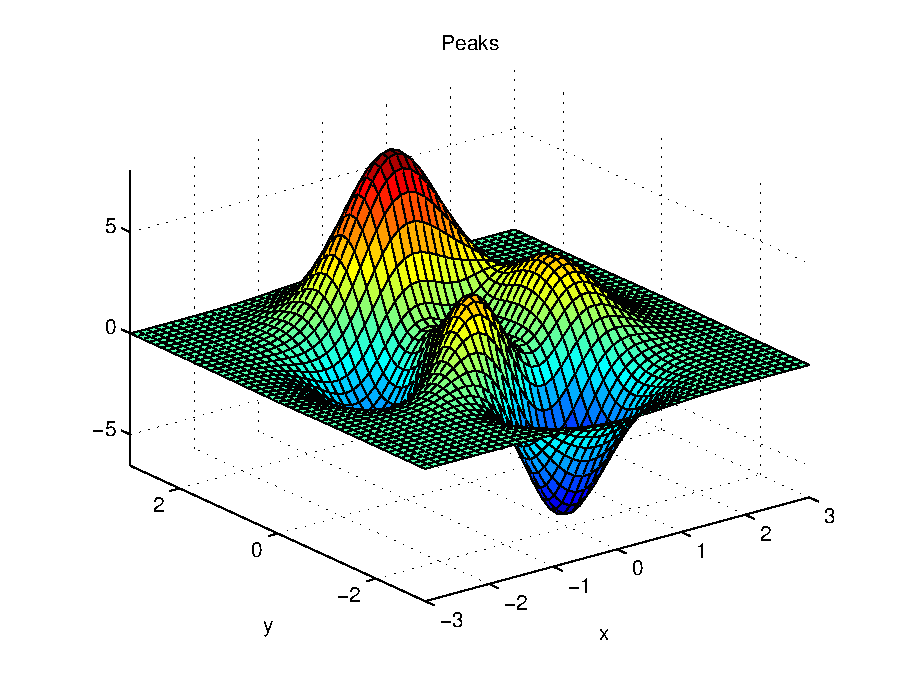
\includegraphics[width=12cm]{example.eps}  % 引入图片源
\caption{example} \label{fig:example}  % 标题与标签
\end{figure}  % 图片结束

This is Figure \eqref{fig:example}.  % 引用图表

This is a cite\cite{vaswani2017attention}.  % 引用文献

\begin{equation}  % 公式,独占一行、居中,自动编号
E = mc^2 \label{aa}  % 标签
\end{equation}  % 公式结束

\begin{equation}  % 公式,独占一行、居中
\nonumber % 不编号
E = mc^2
\end{equation}  % 公式结束

%%%%%%%%%%%%%%%%%%%%%%%% 并排图 %%%%%%%%%%%%%%%%%%%%%%%%
\begin{figure}[h]  % 图片
\centering  % 居中
\begin{minipage}[c]{0.48\textwidth}  % 子页
\centering  % 居中
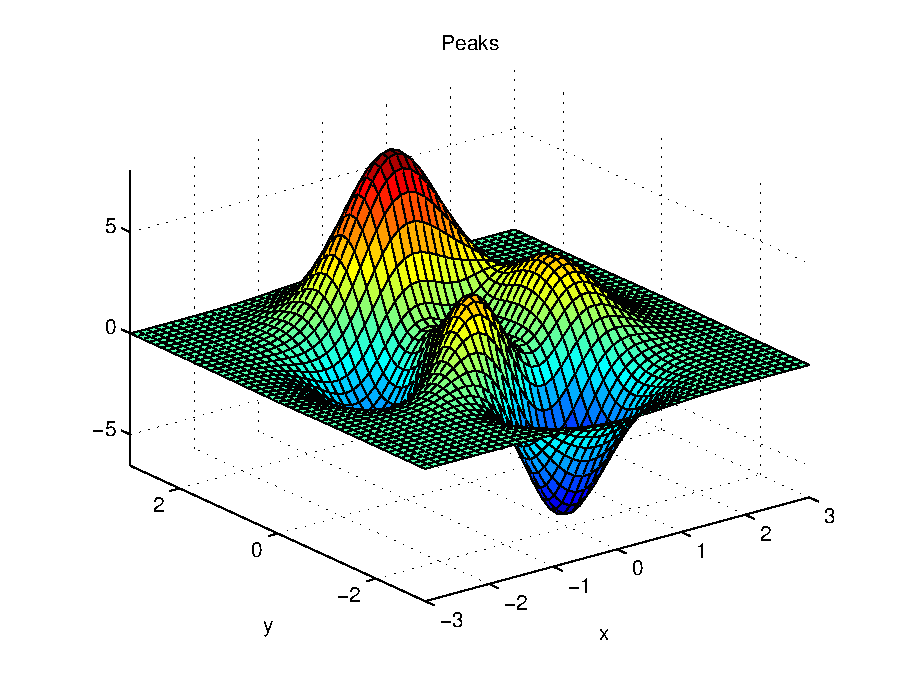
\includegraphics[width=7cm]{example.eps}  % 引入图片源
\caption{example} \label{fig:example}  % 标题与标签
\end{minipage}  % 子页结束
\hspace{0.02\textwidth}
\begin{minipage}[c]{0.48\textwidth}  % 子页
\centering  % 居中
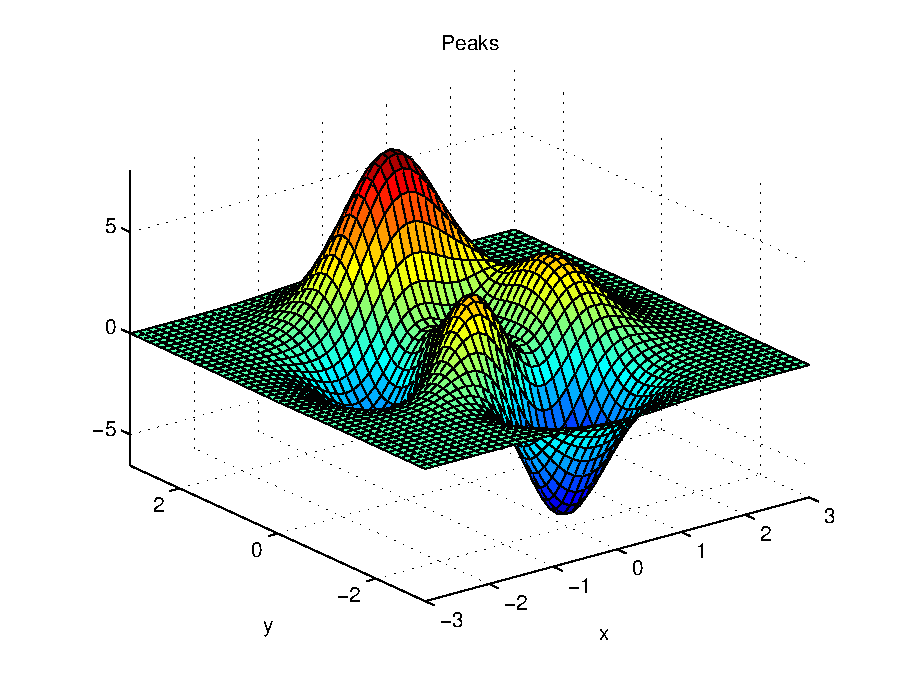
\includegraphics[width=7cm]{example.eps}  % 引入图片源
\caption{example} \label{fig:example}  % 标题与标签
\end{minipage}  % 子页结束
\end{figure}  % 图片结束
%%%%%%%%%%%%%%%%%%%%%% 并排图结束 %%%%%%%%%%%%%%%%%%%%%%

%%%%%%%%%%%%%%%%%%%%%%%% 三线表 %%%%%%%%%%%%%%%%%%%%%%%%
\begin{table}[!t]  % 表格
\caption{Caption}  % 标题
\label{tab1}  % 标签
\tabcolsep 42pt % 列间距
\begin{tabular*}{\textwidth}{cccc}  % tabular*环境
\toprule  % 顶线
Title a & Title b & Title c & Title d \\
\midrule  % 中线
Aaa & Bbb & Ccc & Ddd \\
Aaa & Bbb & Ccc & Ddd \\
Aaa & Bbb & Ccc & Ddd \\
\bottomrule  % 底线
\end{tabular*}  % tabular*环境结束
\end{table}  % 表格结束
%%%%%%%%%%%%%%%%%%%%%% 三线表结束 %%%%%%%%%%%%%%%%%%%%%%

\section{Calculating and Simplifying the Model}  % 一级标题

\section{The Model Results}  % 一级标题

\section{Validating the Model}  % 一级标题

\section{Conclusions}  % 一级标题

\section{Summary}  % 一级标题

\section{Evaluate of the Mode}  % 一级标题

\section{Strengths and weaknesses}  % 一级标题

\subsection{Strengths}  % 二级标题

\newpage
\printbibliography  % 打印引用文献列表

%%%%%%%%%%%%%%%%%%%%%%% 正文结束 %%%%%%%%%%%%%%%%%%%%%%%

\newpage
\begin{appendices}  % 附录

\begin{memo}[Memorandum]  % 建议书
	This is a memorandum.
\end{memo}  % 建议书结束

\section{First appendix}  % 一级标题

Here are simulation programmes we used in our model as follow.\\
\textbf{MATLAB source code:}
\lstinputlisting[language=C++]{./code/main.cpp}

\section{Second appendix}  % 一级标题

\textbf{Python source code:}
\lstinputlisting[language=python]{./code/python.py}

\end{appendices}  % 附录结束
\end{document}  % 文档结束
%%%%%%%%%%%%%%%%%%%%%%%%%%%%%%%%%%%%%%%%%%%%%%%%%%%%%%%
